\section{Reconstruction results}
We will now take a look at some image reconstructions obtained by performing filtered back projection. This has been done in python with the \textit{skimage} library.\\
\begin{figure}
	\centering
	\begin{subfigure}{0.48\linewidth}
		\centering
		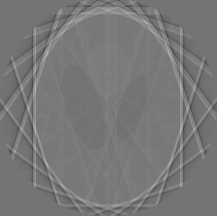
\includegraphics[width=\linewidth]{Materials/recon10}
		\caption{Reconstruction of the Shepp-Logan phantom with 10 angles taken between 0 and 180 degrees.}
	\end{subfigure}
	\hfill
	\begin{subfigure}{0.48\linewidth}
		\centering
		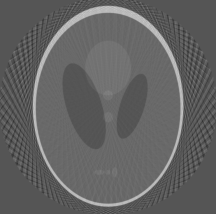
\includegraphics[width=\linewidth]{Materials/recon45}
		\caption{Reconstruction of the Shepp-Logan phantom with 45 angles taken between 0 and 180 degrees.}
	\end{subfigure}
	\\
	\begin{subfigure}{0.48\linewidth}
		\centering
		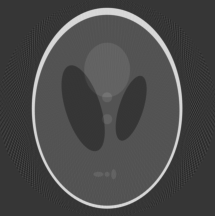
\includegraphics[width=\linewidth]{Materials/recon100}
		\caption{Reconstruction of the Shepp-Logan phantom with 100 angles taken between 0 and 180 degrees.}
	\end{subfigure}
	\hfill
	\begin{subfigure}{0.48\linewidth}
		\centering
		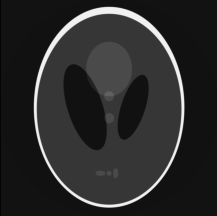
\includegraphics[width=\linewidth]{Materials/recon360}
		\caption{Reconstruction of the Shepp-Logan phantom with 360 angles taken between 0 and 180 degrees.}
	\end{subfigure}
	\caption{Reconstructions of the Shepp-Logan phantom with varying number of projections used.}
	\label{recons}
\end{figure}
In \autoref{recons} we see four image reconstructions of the Shepp-Logan phantom where we have used a varying number of projections to achieve the reconstruction. We see with only 10 projections the most prominent features, namely the big white oval and the two darker ovals in the middle, are reconstructed. However, we also see big artefacts. Using 45 projections we obtain all features of the original image, however, the reconstruction still has a lot of artefacts now seen as a chequerboard patterns around the reconstructed object. Using 100 projections we now have almost no artefacts, and the reconstruction is almost identical to the original image, just brighter and slightly blurred. With 360 projections the artefacts seems to be gone and the reconstruction is \textit{very} close to the original the only differences is the reconstruction is \textit{slightly} blurred and a bit brighter.\\
Comparing \autoref{reconbackprojection} and the reconstructions in \autoref{recons} we see a huge improvement in sharpness and detail.\\
The filtered back projection is a linear reconstruction technique, and thus we can also achieve a complete reconstruction from a sum of reconstructions. By constructing four reconstructions, each consisting of 45 angles, and having them reconstruct one quadrant each, i.e. the first reconstructs 0-45 degrees, the second 45-90 degrees and so on, we can achieve a complete reconstructions by summing the results. The partial reconstructions can be seen in \autoref{partials} and the complete reconstruction can be seen in \autoref{complete}. We see the complete reconstruction is practically identically with the reconstruction obtained in \autoref{recons} where 360 angles were used.
\begin{figure}
	\centering
	\begin{subfigure}{0.48\linewidth}
		\centering
		
\includegraphics[width=\linewidth]{Materials/lin1}
		\caption{Reconstruction of the Shepp-Logan phantom with 45 angles taken between 0 and 45 degrees.}
	\end{subfigure}
	\hfill
	\begin{subfigure}{0.48\linewidth}
		\centering
		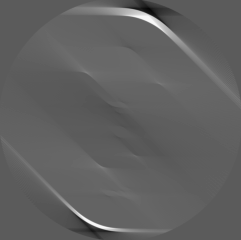
\includegraphics[width=\linewidth]{Materials/lin2}
		\caption{Reconstruction of the Shepp-Logan phantom with 45 angles taken between 45 and 90 degrees.}
	\end{subfigure}
	\\
	\begin{subfigure}{0.48\linewidth}
		\centering
		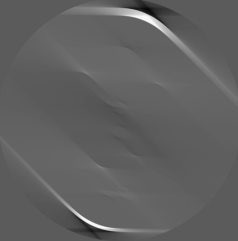
\includegraphics[width=\linewidth]{Materials/lin3}
		\caption{Reconstruction of the Shepp-Logan phantom with 45 angles taken between 90 and 135 degrees.}
	\end{subfigure}
	\hfill
	\begin{subfigure}{0.48\linewidth}
		\centering
		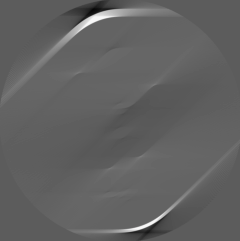
\includegraphics[width=\linewidth]{Materials/lin4}
		\caption{Reconstruction of the Shepp-Logan phantom with 45 angles taken between 135 and 180 degrees.}
	\end{subfigure}
	\caption{Reconstructions of the Shepp-Logan phantom each a reconstruction of a quadrant.}
	\label{partials}
\end{figure}
\begin{figure}
	\centering
	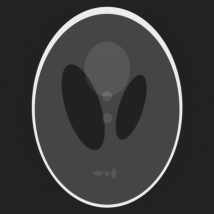
\includegraphics[width=0.5\linewidth]{Materials/complete}
	\caption{The complete reconstruction obtained by adding the four partial reconstructions together.}
	\label{complete}
\end{figure}